\documentclass{beamer}

\usetheme{CambridgeUS}

\usepackage{pacchetticomandi0.14}
% \usepackage{graphicx}
\DeclareMathOperator{\ICM}{ICM}

%AUTHOR DETAILS
%%%%%%%%%%%%%%%%%%%%%%%%%%%%%%%%%%%%%%%%%%%%%%%%
\title[]{Isomorphism classes of principally polarized abelian varieties over finite fields}
\author[Marseglia Stefano]{Marseglia Stefano}
\institute[]{Stockholms Universitet}
\date{22 December 2015}

\begin{document}

\begin{frame}
\titlepage
\end{frame}

% \begin{frame}{Summary of the talk}
% \begin{itemize}
%  \item What is an abelian variety;
%  \item What is the dual abelian variety;
%  \item What is a polarization;
%  \item Deligne category;
%  \item Why compute the $\ICM$;
%  \item Weak equivalent classes;
%  \item Isomorphisms Classes;
%  \item Howe's description;
%  \item Polarizations;
% \end{itemize}
% \end{frame}

\begin{frame}{Abelian varieties}

  \begin{block}{Definition}
    An \textbf{abelian variety $A$} over a field $k$ is a connected and complete group variety over $k$, that is a $k$-variety $A$ together with morphisms $m:A \times A \to A$ and $\iota: A \to A$ and a identity element $e\in A(k)$ such that the quadruple $(A,m,\iota, e)$ is a group in the category of varieties.
  \end{block}
\pause
  It turns out that:
  \begin{itemize}
   \item $A$ is non-singular;
   \item $A$ is projective;
   \item the group law on $A$ is commutative;
   \item a morphism $f:A\to B$ is the composition of homomorphism $h: A \to B$ and a translation $t_b$, for some $b=-f(e_A)\in B(k)$.
  \end{itemize}
\end{frame}

\begin{frame}{Example}
    One-dimensional abelian varieties are called \textbf{elliptic curves}.
\pause    
  \begin{exampleblock}{Example}
    If $\Char(k) \neq 2,3$ consider $\cC: y^2=x^3+ax+b$, with $4a^3+27b^2 \neq 0$.\\
    In this case we can describe explicitly the group law:\\
    \begin{figure}
        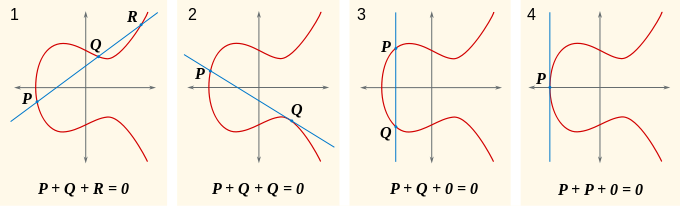
\includegraphics[width=1\textwidth]{ECgrouplaw}
        \caption{www.limited-entropy.com}
    \end{figure}
  \end{exampleblock}
\end{frame}

\begin{frame}{Isogenies}
  \begin{block}{Definition}
    A homomorphism $f:A\to B$ is called \textbf{isogeny} if it is surjective and with finite kernel. The \textbf{degree} of $f$ is the degree of the kernel of $f$ (as a finite group scheme).
  \end{block}
\pause
  In particular:
  \begin{itemize}
    \item if $A\simeq B$ then $\dim A = \dim B$;
    \item $\deg(f\circ g) = \deg(f)\deg(g)$;
    \item if $\deg(f)=n$ then there exists an isogeny $g:B \to A$ such that $f\circ g = n_A: a \mapsto na$ for every $a\in A(k)$;
    \item $A\simeq \prod_i A_i^{e_i}$, with the $A_i$'s are \textbf{simple} and non-isogenous.
  \end{itemize}
\end{frame}

\begin{frame}{Dual abelian variety}
  Put: $\Pic^0(A) = \set{\cL \text{ inv. sheaf : }t^*_a\cL\approx\cL \text{ on }A_{\bar k} \text{ for all }a\in A(\bar k) }/\approx.$
  \begin{block}{Definition}
    An abelian variety $A^\vee$ is the \textbf{dual} abelian variety of $A$ and an invertible sheaf $\cP$ on $A\times A^\vee$ is the \textbf{Poincar\`e} sheaf if:
    \begin{enumerate}
      \pause \item $\cP|_{\set{e}\times A^\vee}$ is trivial and $\cP|_{A\times \set{a}}$ lies in $\Pic^0(A_{k(a)})$ for all $a\in A^\vee$; and
      \pause \item for every $k$-scheme $T$ and invertible sheaf $\cL$ on $A\times T$ such that $\cL|_{\set{e}\times A^\vee}$ is trivial and $\cL|_{A\times \set{t}}$ lies in $\Pic^0(A_{k(t)})$ for all $t\in T$, there is a unique morphism $f:T\to A^\vee$ such that $(1\times f)^*\cP\approx \cL$.
    \end{enumerate}
  \end{block}
\end{frame}

\begin{frame}{Polarizations}
  In particular:
  \begin{itemize}
    \item $(A^\vee,\cP)$ is uniquely determined up to a unique isomorphism;
    \item $A^\vee(\bar k) = \Pic^0(A_{\bar k})$ and every element of $\Pic^0(A_{\bar k})$ is represented uniquely once in the family $(\cP_a)_{a\in A(\bar k)}$;
    \item $A^{\vee\vee} = A$.
  \end{itemize}
\pause
  \begin{block}{Definition}
    A \textbf{polarization} $\lambda$ on $A$ is an isogeny $\lambda: A\to A^\vee$ such that $\lambda_{\bar k}=\vphi_\cL: a\mapsto t_a^*\cL \otimes \cL^{-1}$ for some ample invertible sheaf $\cL$ on $A_{\bar k}$.\\
    If $\deg(\lambda)=1$ we say that $A$ is \textbf{principally polarized}.
  \end{block}
  \begin{itemize}
     \pause \item The automorphism group of $(A,\lambda)$ is finite.
  \end{itemize}
\end{frame}

\begin{frame}{Over $k=\C$ ...}
  If $k= \C$ the situation is simpler!\\
\pause
  An abelian variety over $\C$ of dimension $g$ is a \textbf{complex torus} $A=V/\Lambda$  with a \textbf{non-degenarete Riemann form} $H:V\times V \to \C$, where:
\pause
  \begin{itemize}
    \item $V = $ a $g$-dimensional $\C$-vector space;
    \item $\Lambda =$ a lattice of rank $2g$ (inside $V$);
    \item $H$ is Hermitian and $E=\Im H$ is integer valued on $\Lambda$.
  \end{itemize}
\pause
  The \textbf{dual} variety is $A^\vee = V^*/\Lambda^*$, where:
  \begin{itemize}
    \item $V^* = {\text{antilinear functionals on } V }$, and
    \item $\Lambda^* = \set{f\in V^* | \Span{f,t}:=\Im(f(t)) \in \Z \text{ for all }t\in \Lambda}$.
  \end{itemize}
\pause
  A \textbf{polarization} is an equivalence class of Riemann forms (containing a non-degenerate one), where $H_1\sim H_2 \Longleftrightarrow \exists n_1,n_2\in \N: n_1H_1=n_2H_2$.
\end{frame}

\begin{frame}{... and in $\Char(k)=p>0$}

  \begin{itemize}
    \pause \item Serre: when $\Char(k)=p>0$ it is \textbf{not} possible to functorially attach a free abelian group of rank $2g$ to a $g$-dimensional abelian variety $A$.
    \pause \item Weil: for $l\neq p$: $A[l^m](\bar k)\simeq (\Z/l^m\Z)^{2g}$;
    \pause \item but: $A[p^m](\bar k)\simeq (\Z/p^m\Z)^{f}$ for some $0\leq f \leq g$.
  \end{itemize}
\end{frame}

\begin{frame}{Frobenius}
  Let's move to finite fields:
\pause
  \begin{block}{Definition}
    Let $A$ be an abelian variety over $\F_q$. The \textbf{Frobenius} morphism of $A$ is the morphism $\pi_A:A\to A$ which is the identity on the underlying topological space and is the map $x\mapsto x^q$ on $\cO_A$. It is an isogeny of degree $q$.
  \end{block}
\pause
  \begin{alertblock}{Theorem}
    Let $h_A$ be the \textbf{characteristic} polynomial of $\pi_A$ (on $T_lA:= \varprojlim A[l^m](\bar k)$).
    Write $h_A(X)=\prod_{i=0}^{2g}(X-\alpha_i)$. The roots $\alpha_i$ are called \textbf{$q$-Weil numbers}. Then
 \pause   
    \begin{itemize}
      \item $h_A(X)\in \Z[X]$;
      \item $\# A(\F_{q^m})=\prod(1-\alpha_i^m)$, for all $m\geq 1$;
      \item $\abs{\alpha_i}=\sqrt{q}$.
    \end{itemize}
  \end{alertblock}
\end{frame}

\begin{frame}{Classification up to isogeny: Honda-Tate theory}
  \begin{alertblock}{Theorem (Tate)}
    The abelian varieties $A$ and $B$ over $\F_q$ are isogenous if and only if $h_A = h_B$.
  \end{alertblock}
\pause
  Recall: two algebraic numbers $\alpha$ and $\beta$ are conjugate if and only if $\Q(\alpha)\simeq \Q(\beta)$.
  \begin{alertblock}{Theorem (Honda)}
    There is a bijection between conjugacy classes of $q$-Weil numbers and isogeny classes of simple abelian varieties over $\F_q$
  \end{alertblock}
\end{frame}

\begin{frame}{Deligne's category}
  \begin{block}{Definition}
    We say that $A$ is \textbf{ordinary} if one of the following equivalent
    conditions holds:
\pause
    \begin{itemize}
      \item $\#A[p](\bar k) = p^g$;
      \item exactly half of the roots of $h_A$ are $p$-adic units;
      \item the middle coefficient of $h_A$ is coprime to $p$.
    \end{itemize}
  \end{block}
\pause
  \begin{block}{Definition}
    Let $\cD_q$ be the category of pairs $(T,F)$, with
    \begin{itemize}
      \item $T$ is a free $\Z$-module of even rank and $F$ is an endomorphism of $T$;
      \item $F\otimes \Q$ is semi-simple and its eigenvalues have complex-size $\sqrt{q}$;
      \item half of the roots of the characteristic polynomial of $F$ are $p$-adic units;
      \item exists an endomorphism $V$ such that $FV=q$.
    \end{itemize}
  \end{block}
\end{frame}

\begin{frame}{Construction of the equivalence}
  \begin{alertblock}{Theorem (Deligne ('69))}
    There is an equivalence of categories $T$ between the category of ordinary abelian varieties over $\F_q$ and $\cD_q$.
  \end{alertblock}
  \begin{itemize}
    \pause \item Let $\tilde A$ be the canonical Serre-Tate lift of $A$ to the ring of Witt-vectors $W(\overline{\F}_q)$;
    \pause \item choose and embedding $\varepsilon: W(\overline{\F}_q)\hookrightarrow \C$;
    \pause \item define $T(A):=H_1(\tilde A \otimes_\epsilon \C)$ and $F$ the lift of $\pi_A$.
  \end{itemize}
\pause
  Observe: $\rk (T(A)) = 2\dim(A)$

  and $T(\pi_A)=F(A)$.
\pause
\end{frame}

\begin{frame}{Dual varieties in $\cD_q$}
\pause
  \begin{block}{Definition}
    The \textbf{dual} of $(T,F)\in \cD_q$ is $(\hat T,\hat F)$, where
    \begin{itemize}
      \item $\hat T = \Hom_\Z(T,\Z)$;
      \item $\hat F: \psi \mapsto \psi\circ V$.
    \end{itemize}
  \end{block}
\pause
  \begin{alertblock}{Theorem (Howe '95)}
    Deligne's equivalence respects duality.
  \end{alertblock}
\end{frame}

\begin{frame}{Polarizations in $\cD_q$}
  Let $(T,F) \in \cD_q$. Put $R=\Z[F,V]\subseteq \End((T,F))$.\\
\pause
  Observe: $K=R\otimes \Q$ is a product of CM-fields.\\
\pause
  Let $v$ be the $p$-adic valuation induced by the embedding $\varepsilon: W(\overline \F_q)\hookrightarrow \C$.\\
\pause
  Define the CM-type $\Phi:=\set{\vphi:K\to \C | v(\vphi(F))>0}$.\\
\pause
  Let $\iota \in K$ such that $\vphi(\iota)$ is positive imaginary for every $\vphi \in \Phi$.\\
\pause
  Fact: an isogeny $\lambda: (T,F) \to (\hat T, \hat F)$ induces a pairing $b:T\times T \to \Z$.
\pause
  \begin{block}{Definition}
    The isogeny $\lambda$ is a \textbf{polarization} if:
    \begin{itemize}
      \item $b$ is alternating, and
      \item the pairing $(x,y)\mapsto b(\iota x,y)$ on $T\times T$ is symmetric and positive definite.
    \end{itemize}
  \end{block}
\pause
  \begin{alertblock}{Theorem (Howe '95)}
    Deligne's equivalence sends polarizations to polarizations.
  \end{alertblock}
\end{frame}

\begin{frame}{When $h$ is irreducible}
  Fix an irreducible ordinary $q$-Weil polynomial $h$ and let $F$ be a root.\\
\pause
  Let $\cI$ be the isogeny class corresponding to $h$ in $\cD_q$.\\
\pause
  Put $R=\Z[F,V]$. It is an order in the number field $K=\Q[X]/h(X)$.\\
\pause
  \begin{alertblock}{Proposition (Howe)}
    \[\set{\text{Deligne modules in $\cI$}} \longleftrightarrow \set{\text{Fractional ideals of $R$}} \]
\pause
    Let $I$ be a fractional $R$-ideal corresponding to a Deligne module $(T,F)$.\\
\pause
    Then $(\hat T, \hat F)$ corresponds to $\overline I ^t$, where $I^t=\set{x\in K:\Tr_{K/\Q}(xI)\subseteq \Z}$ is the \textbf{trace dual} of $I$ and $\overline{\cdot}$ is the CM-conjugation of $K$.\\
\pause
    Moreover a \textbf{polarization} of $(T,F)$ is $\lambda\in K^*$ such that
    \begin{itemize}
      \item $\lambda I \subseteq \overline I^t$;
      \item $\lambda$ is totally imaginary;
      \item $\vphi(\lambda)$ is positive imaginary for every $\vphi \in \Phi$.
    \end{itemize}
  \end{alertblock}
\end{frame}

\begin{frame}{Isomorphism classes}
  Goal: count the isomorphism classes, with polarizations.\\
\pause
  We get
  \[\set{\parbox[p]{9.5em}{Isomorphism classes of \\abelian varieties in $\cI$}} \longleftrightarrow \set{\textbf{Ideal class monoid} \text{ of $R$}}
\]

  Recall: $I \simeq J \Longleftrightarrow \exists x\in K^* : I=xJ$.\\
\pause
  Problem: it is not known how to compute efficiently the $\ICM(R)$ when $R$ is not maximal (not Dedekind), because there are \textbf{non-invertible classes}.\\
\pause
  Let $[I]\in ICM(R)$ such that $x I = \overline I^t$ for some $x\in K^*$.\\
\pause
  If for some $u\in (I:I)^\times$ we have $xu$ is totally imaginary and $\vphi(xu)$ is positive imaginary for every $\vphi \in \Phi$ then $\lambda:=xu$ is a polarization of $I$.
\end{frame}

\begin{frame}{Number of polarizations and automorphisms}
  Assume that $I$ has a polarization $\lambda$. Then:
\pause
  \[
    \set{\parbox[p]{11em}{number of non-isomorphic \\ polarizations on $I$}} \longleftrightarrow
    \dfrac{\set{ \text{totally positive $u\in (I:I)^\times$} }}{\set{v\bar v : v\in (I:I)^\times}}
  \]
\pause
  and 
  \[
    \Aut((I,\lambda)) \longleftrightarrow
    \set{\text{torsion units }u\in (I:I)^\times}
  \]
\end{frame}

\begin{frame}{Computations}
  Abelian surfaces over $\F_3$ with \textbf{irreducible ordinary (and Clifford)} polynomials:
\pause
  \begin{align*}
    & x^4 - 4x^3 + 8x^2 - 12x + 9 = [ 8 ] &
    & x^4 - 3x^3 + 5x^2 - 9x + 9 = [ 2 ]\\
    & x^4 - 2x^3 + x^2 - 6x + 9 = [ 6 ] &
    & x^4 - 2x^3 + 2x^2 - 6x + 9 = [ 2, 4 ]\\
    & x^4 - 2x^3 + 4x^2 - 6x + 9 = [ 2, 2 ] &
    & x^4 - 2x^3 + 5x^2 - 6x + 9 = [ 2 ]\\
    & x^4 - x^3 - 2x^2 - 3x + 9 = [ 6 ] &
    & x^4 - x^3 - x^2 - 3x + 9 = [ 2 ]\\
    & x^4 - x^3 + 2x^2 - 3x + 9 = [ 2, 2 ] &
    & x^4 - x^3 + 5x^2 - 3x + 9 = [ 2 ]\\
    & x^4 - 5x^2 + 9 = [ 4 ] &
    & x^4 - x^2 + 9 = [ 2, 2 ]\\
    & x^4 + x^2 + 9 = [ 2, 2 ] &
    & x^4 + x^3 - 2x^2 + 3x + 9 = [ 6 ]\\
    & x^4 + x^3 - x^2 + 3x + 9 = [ 2 ] &
    & x^4 + x^3 + 2x^2 + 3x + 9 = [ 2, 2 ]\\
    & x^4 + x^3 + 5x^2 + 3x + 9 = [ 2 ] &
    & x^4 + 2x^3 + x^2 + 6x + 9 = [ 6 ]\\
    % & x^4 + 2x^3 + 2x^2 + 6x + 9 = [ 2, 4 ] &
    % & x^4 + 2x^3 + 4x^2 + 6x + 9 = [ 2, 2 ]\\
    & \cdots
    % & x^4 + 2x^3 + 5x^2 + 6x + 9 = [ 2 ]
    % & x^4 + 3x^3 + 5x^2 + 9x + 9 = [ 2 ]\\
    % & x^4 + 4x^3 + 8x^2 + 12x + 9 = [ 8 ]
  \end{align*}
\end{frame}

% \begin{frame}{How to compute the $\ICM$}
% 
% \end{frame}

% \begin{block}{Definition}
% 
% \end{block}

% \begin{alertblock}{Proposition}
% 
% \end{alertblock}

% \begin{exampleblock}{Example}
% 
% \end{exampleblock}

% \begin{frame}{???}
% 
% \end{frame}



% \begin{itemize}
% \pause \item ???
% \pause \item ???
% \end{itemize}

\begin{frame}
\begin{center}
{\LARGE \textit{Thank you for your attention.}}
\end{center}
\end{frame}

\end{document}